\begin{exercise}{Mélange d'acide et d'eau de javel}{2}{PCSI}{Chimie générale, Oxydoréduction, Diagramme de E-pH}{chocron}

On dit souvent qu'il ne faut pas mélanger les produits ménagers, c'est en particulier le cas de l'eau de Javel  avec tout produit acide. Essayons de comprendre pourquoi. Le gaz dichlore est un gaz toxique irritant, pouvant entraîner des problèmes pulmonaires graves en cas d'inhalation. Une solution aqueuse de dichlore Cl$_{2(aq)}$ peut libérer du dichlore Cl$_{2(g)}$ gazeux. L'eau de Javel est une solution aqueuse comportant du chlorure de sodium (Na$^+$ + Cl$^-$) et de l'hypochlorite de sodium (Na$^+$ + ClO$^-$) en quantité équimolaire. Le diagramme potentiel-pH simplifié de l'élément chlore est représenté en annexe, pour les espèces chimiques HClO$_{(aq)}$, ClO$^-_{(aq)}$, Cl$_{2(aq)}$ et Cl$^-_{(aq)}$. \'A la frontière entre deux domaines, on suppose l'équirépartition en \textbf{élément} chlore. 

\begin{questions}
\question Attribuer chacun des domaines A, B, C et D à une espèce mentionnée ci-dessus.

\question En vous aidant du diagramme et des données, déterminer la valeur de C$_0$, concentration de tracé qui est la concentration totale en \textbf{élément} chlore; déterminer également la valeur du pK$_a$ du couple HClO/ClO$^-$.

\question Déterminer les pentes des frontières entre les domaines A et B, A et C ainsi que D et C. 

\question En utilisant le diagramme E-pH, prévoir l'évolution d'un mélange contenant les espèces D et C lors du passage en milieu très acide. \'A partir de quel pH observe-t-on cette réaction?

\question Donner l'équation de cette réaction et calculer sa constante d'équilibre à 298K. Comment s'appelle la réaction mise en jeu? 

\question  Conclure quant à la consigne de sécurité figurant sur les flacons d'eau de Javel de ne pas mélanger un acide avec de l'eau de Javel. 

\end{questions}
\begin{figure}[H]
    \centering
    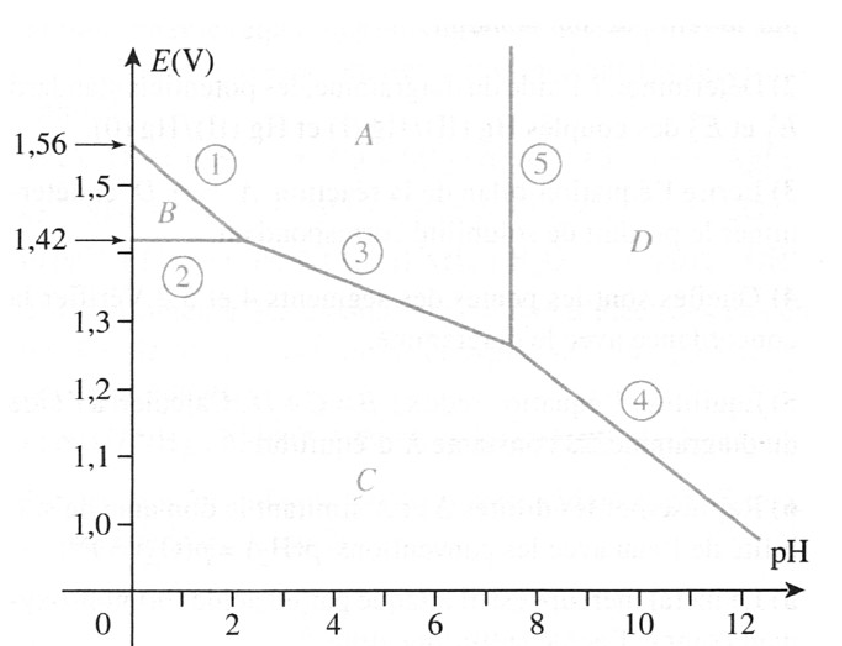
\includegraphics{chimiePC/gene/e-ph_chlore.pdf}
    \caption{Diagramme E-pH du chlore}
   
\end{figure}

\paragraph{Données : } potentiels standards $E^\circ$ dans les CNTP
\begin{center}\begin{tabularx}{.7\linewidth}{rCCC}
    \hline
    & $\mathrm{{HClO}_{(aq)} \,/\, {Cl_2}_{(aq)}}$
    & $\mathrm{{Cl_2}_{(aq)} \,/\, {Cl^-}_{(aq)}}$
    & $\mathrm{{O_2}_{(g)} \,/\, {H_2O}_{(\ell)}}$ \\
    $E^\circ$ (V) & 1,60 & 1,39 & 1,23 \\
    $E^\circ / \varepsilon^\circ$ & 27 & 24 & 21 \\ \hline\hline 
\end{tabularx}
\end{center}

On note $\varepsilon^\circ = \dfrac{RT}{\scr{F}} \ln10 = 59$ mV.


\end{exercise}


\begin{solution}

\begin{questions}
\question 
D.O. du chlore : 
Cl$_2$ : 0
Cl$^-$ : $-$I
HClO et ClO$^-$ : +I

On a donc C : Cl$^-$ ; B : Cl$_2$ ; A : HClO (espèce acide) ; D : ClO$^-$ (espèce basique).


\question  On se place à la frontière horizontale entre B et C qui correspond à la frontière entre Cl$^-$ et Cl$_2$.

La demi-équation redox correspondante est : Cl$_2$ + 2e$^-$ = 2Cl$^-$
Au niveau de cette frontière, la formule de Nernst donne : 
$E = E^\circ(Cl_{2(aq)}/Cl^-_{(aq)}) + \frac{0,06}{2}log(\frac{[Cl_2]}{[Cl^-]^2}$. 

A la frontière, l'équirépartition en chlore s'écrit : 2[Cl$_2$]=[Cl$^-$] et on a 2[Cl$_2$] + [Cl$^-$] = C$_0$.

Cela donne donc $E = E^\circ(Cl_{2(aq)}/Cl^-_{(aq)}) + 0,03log(\frac{1}{C_0})$ d'où avec les valeurs numériques des données et lue sur le diagramme, C$_0$ = 10$^{-1}$ mol.L$^{-1}$

La frontière verticale entre A et D représente l'équilibre acido-basique du couple HClO/ClO$^-$. A la frontière, on a $K_a=\frac{[ClO^-]\times[H^+]}{[HClO]}$ et [ClO$^-$]=[HClO] d'où $K_a= [H^+] $ ie $pK_a(HClO/ClO^-) = pH_{frontière}$ = 7,5.

\question La frontière entre A et B est la frontière du couple HClO/Cl$_2$ de demi-équation redox 2HClO + 2H$^+$ + 2e$^-$ = Cl$_2$ + 2H$_2$0

D'où en utilisant la formule de Nernst la pente vaut -0,06 V.

Pour A et C, on considère le couple HClO/Cl$^-$ de demi-équation HClO + H$^+$ + 2e$^-$ = Cl$^-$ + H$_2$O. La pente vaut -0,03 V.

Pour D et C, on considère le couple ClO$^-$/Cl$^-$ de demi-équation ClO$^-$ + 2H$^+$ + 2e$^-$ = Cl$^-$ + H$_2$O. La pente vaut -0,06 V.


\question Lorsque on modifie le pH d'une solution d'eau de javel (mélange de Cl$^-$ et ClO$^-$) à un pH inférieur à 2,5, HClO et Cl$^-$ n'ont plus de frontière commune donc vont réagir ensemble pour former du dichlore. A un pH inférieur à 7,5 ClO$^-$ n'est plus la forme prédominante du couple HClO/ClO$^-$.

\question Si on part d'une solution d'eau de Javel, les espèces en présence sont ClO$^-$ et Cl$^-$ donc on va considérer la réaction de ces deux espèces selon l'équation : Cl$^-$ + ClO$^-$ + 2H$^+ \rightleftarrows$ Cl$_2$ + H$_2$O. Il s'agit d'une réaction de médiamutation. 

Avec les données, on peut calculer la constante d'équilibre de la réaction 

Cl$^-$ + HClO + H$^+ \rightleftarrows$ Cl$_2$ + H$_2$O qui vaut $K_1 = 10^{\frac{E^\circ(HClO/Cl_2)-E^\circ(Cl_2/Cl^-)}{0,06}} = 10^{3,5}$ et $K$ la constante d'équilibre de la réaction avec ClO$^-$ vaut $\frac{K_1}{K_a} = 10^{3,5+7,5} = 10^{11}$.


\question On voit que la constante d'équilibre est élevée, la réaction est quantitative. Le mélange d'eau de Javel avec un acide conduit à la formation de dichlore aqueux, qui passe ensuite sous forme gazeuse. Le dichlore est un gaz très toxique, les indications sur les bouteilles sont donc tout à fait justifiées

\end{questions}
\end{solution}